% Template for Cogsci submission with R Markdown

% Stuff changed from original Markdown PLOS Template
\documentclass[10pt, letterpaper]{article}

\usepackage{cogsci}
\usepackage{pslatex}
\usepackage{float}
\usepackage{caption}

% amsmath package, useful for mathematical formulas
\usepackage{amsmath}

% amssymb package, useful for mathematical symbols
\usepackage{amssymb}

% hyperref package, useful for hyperlinks
\usepackage{hyperref}

% graphicx package, useful for including eps and pdf graphics
% include graphics with the command \includegraphics
\usepackage{graphicx}

% Sweave(-like)
\usepackage{fancyvrb}
\DefineVerbatimEnvironment{Sinput}{Verbatim}{fontshape=sl}
\DefineVerbatimEnvironment{Soutput}{Verbatim}{}
\DefineVerbatimEnvironment{Scode}{Verbatim}{fontshape=sl}
\newenvironment{Schunk}{}{}
\DefineVerbatimEnvironment{Code}{Verbatim}{}
\DefineVerbatimEnvironment{CodeInput}{Verbatim}{fontshape=sl}
\DefineVerbatimEnvironment{CodeOutput}{Verbatim}{}
\newenvironment{CodeChunk}{}{}

% cite package, to clean up citations in the main text. Do not remove.
\usepackage{apacite}

% KM added 1/4/18 to allow control of blind submission


\usepackage{color}

% Use doublespacing - comment out for single spacing
%\usepackage{setspace}
%\doublespacing


% % Text layout
% \topmargin 0.0cm
% \oddsidemargin 0.5cm
% \evensidemargin 0.5cm
% \textwidth 16cm
% \textheight 21cm

\title{Peekbank: Exploring child lexical processing through a large-scale
open-source database of developmental eyetracking datasets}


\author{{\large \bf Martin Zettersten (martincz@princeton.edu)} \\ Department of Psychology, South Dr \\ Princeton, NJ 08540 USA \AND {\large \bf CLinger Xu (txu@iu.edu)}  \AND {\large \bf Claire Bergey (cbergey@uchicago.edu)}  \AND {\large \bf Naiti S. Bhatt (nbhatt@hmc.edu)}  \AND {\large \bf Veronica Boyce (vboyce@stanford.edu)}  \AND {\large \bf Mika Braginsky (mikabr@mit.edu)}  \AND {\large \bf George Kachergis (kachergis@stanford.edu)}  \AND {\large \bf Molly Lewis (mollyllewis@gmail.com)}  \AND {\large \bf Jessica Mankewitz (jmankewitz@stanford.edu)} \AND {\large \bf Stephan Meylan (smeylan@mit.edu)}  \AND {\large \bf Annissa Saleh (ans638@nyu.edu)}  \AND {\large \bf Rose Schneider (roschnei@ucsd.edu)}   \AND {\large \bf Daniel Yurovsky (yurovsky@stanford.edu)}  \AND {\large \bf CMichael C. Frank (mcfrank@stanford.edu)}}


\begin{document}

\maketitle

\begin{abstract}
Developing lexical processing skills - the ability to rapidly process
words and link them to referents in context - is central to children's
early language development. Children's lexical processing is typically
studied in the looking-while-listening paradigm - also called the visual
world paradigm -, which measures infants' fixation of a target object
(as opposed to a distracter) after hearing a target label. In the
following paper, we present a large-scale open-source database of infant
and toddler looking-while-listening studies. The goal of this database
is to address theoretical and methodological challenges in measuring
infant vocabulary development that go beyond the scope of individual
studies. We present three preliminary analyses from the current
database: (1) models capturing item-level variability in infants'
lexical processing across age; (2) an analysis of how a central
methodlogical decision - selecting the time window of analysis - impacts
modeling results; (3) an analysis demonstrating the link between the age
of acquisition of specific words and children's ability to rapidly and
accurately link those words to their referents. Future efforts will
expand the scope of the current database to advance our understanding of
participant-level and item-level variation in children's vocabulary
development.

\textbf{Keywords:}
lexical processing; eyetracking; database; vocabulary development;
looking-while-listening; visual world paradigm
\end{abstract}

\hypertarget{introduction}{%
\section{Introduction}\label{introduction}}

Across their first years of life, children learn words in their native
tongues at a rapid pace. A key part of the word learning process is
children's ability to rapidly process words and link them to relevant
meanings in context - often referred to as lexical processing.
Developing lexical processing skills builds a foundation for children's
language development and is predictive of both linguistic and more
general cognitive outcomes later in life.

\hypertarget{the-success-of-the-looking-while-listening-paradigm}{%
\subsection{The success of the looking-while-listening
paradigm}\label{the-success-of-the-looking-while-listening-paradigm}}

Lexical processing is traditionally studied in
``looking-while-listening'' studies (sometimes called the intermodal
preference procedure). In such studies, infants listen to a sentence
prompting a specific referent (e.g., Look at the dog!) while viewing two
images on the screen (e.g., an image of a dog - the target image - and
an image of a duck - the distractor image). Infants' lexical processing
is measured in terms of how quickly and accurately infants subsequently
fixate the correct target image after hearing its label. Studies using
this basic design have contributed to our understanding of a wide range
of questions in language development, including infants' early noun
knowledge (Bergelson \& Swingley, 2012), phonological representations of
words (Swingley \& Aslin), prediction during language processing
(Lew-Williams; others), individual differences in language development
(xx), and .

\hypertarget{outstanding-challenges}{%
\subsection{Outstanding challenges}\label{outstanding-challenges}}

While the looking-while-listening paradigm has been highly fruitful in
advancing understanding of early word knowledge, fundamental questions
remain both about the nature of children's early word knowledge and the
nature of the method itself. One central question relates to
understanding word-specific variability across development, and
generalizing lexical processing on the level of specific words. Most
studies of infant lexical processing focus on generalizing performance
across participants, and are constrained in their ability to provide
generalizations across the item level - the level of specific words.
Generalizing behavior on the level of both participants and items
simultaneously is often difficult in the context of a solitary study,
especially given practical constraints on the number of trials (and
consequently items) tested within a given infant. However, drawing
inferences about item-level variability is key to many questions in how
word learning unfolds, including how properties of the language input
influence lexical development (Item-based analytic approach - Goodman,
Dale, \& Li (2008), Roy et al.~(2015), Braginsky et al.~(2018) all look
at predicting items from input). One key to meeting this challenge is
having sufficiently large datasets to interrogate variability in lexical
processing on the item level.

A second question relates to evaluating methodological best-practices.
In particular, many fundamental analytic decisions vary substantially
across studies. For example, researchers vary in their decisions
regarding how to select time windows for analysis (XX), modeling how
lexical processing unfolds over time (XX), and the appropriate
transformations to perform on the dependent measure of target fixations.
Establishing best practices regarding analytic decisions of this kind
requires a large database of infant lexical processing studies, in order
to independently test the potential consequences of a variety of
methodological decisions on the interpretation of study results.

\hypertarget{peekbank-a-large-scale-database-of-looking-while-listening-studies}{%
\subsection{Peekbank: A large-scale database of
looking-while-listening-studies}\label{peekbank-a-large-scale-database-of-looking-while-listening-studies}}

What these questions and challenges share is that they are difficult to
answer at the scale of a single looking-while-listening study. In order
to address these questions, we introduce peekbank, a flexible and
reproducible interface to an open database of developmental eye-tracking
studies. Here, we give a brief overview over the key components of the
peekbank project and some initial demonstrations of its utility in
advancing theoretical and methodological questions in the study of
children's lexical processing. The peekbank project (a) collects a large
set of eye-tracking datasets on children's lexical processing, (b)
introduces a data format and processing tools for standardizing
eyetracking data across different data sources, and (c) provides an API
for quickly accessing and analyzing the database.

\hypertarget{methods}{%
\section{Methods}\label{methods}}

First level headings should be in 12 point , initial caps, bold and
centered. Leave one line space above the heading and
1/4\textasciitilde line space below the heading.

\hypertarget{second-level-headings}{%
\subsection{Second-Level Headings}\label{second-level-headings}}

Second level headings should be 11 point , initial caps, bold, and flush
left. Leave one line space above the heading and 1/4\textasciitilde{}
line space below the heading.

\hypertarget{third-level-headings}{%
\subsubsection{Third-Level Headings}\label{third-level-headings}}

Third-level headings should be 10 point , initial caps, bold, and flush
left. Leave one line space above the heading, but no space after the
heading.

\hypertarget{formalities-footnotes-and-floats}{%
\section{Formalities, Footnotes, and
Floats}\label{formalities-footnotes-and-floats}}

Use standard APA citation format. Citations within the text should
include the author's last name and year. If the authors' names are
included in the sentence, place only the year in parentheses, as in
(1972), but otherwise place the entire reference in parentheses with the
authors and year separated by a comma (Newell \& Simon, 1972). List
multiple references alphabetically and separate them by semicolons
(Chalnick \& Billman, 1988; Newell \& Simon, 1972). Use the et.
al.~construction only after listing all the authors to a publication in
an earlier reference and for citations with four or more authors.

For more information on citations in RMarkdown, see
\textbf{\href{http://rmarkdown.rstudio.com/authoring_bibliographies_and_citations.html\#citations}{here}.}

\hypertarget{footnotes}{%
\subsection{Footnotes}\label{footnotes}}

Indicate footnotes with a number\footnote{Sample of the first
footnote.} in the text. Place the footnotes in 9 point type at the
bottom of the page on which they appear. Precede the footnote with a
horizontal rule.\footnote{Sample of the second footnote.} You can also
use markdown formatting to include footnotes using this
syntax.\footnote{Sample of a markdown footnote.}

\hypertarget{figures}{%
\subsection{Figures}\label{figures}}

All artwork must be very dark for purposes of reproduction and should
not be hand drawn. Number figures sequentially, placing the figure
number and caption, in 10 point, after the figure with one line space
above the caption and one line space below it. If necessary, leave extra
white space at the bottom of the page to avoid splitting the figure and
figure caption. You may float figures to the top or bottom of a column,
or set wide figures across both columns.

\hypertarget{two-column-images}{%
\subsection{Two-column images}\label{two-column-images}}

You can read local images using png package for example and plot it like
a regular plot using grid.raster from the grid package. With this method
you have full control of the size of your image. \textbf{Note: Image
must be in .png file format for the readPNG function to work.}

You might want to display a wide figure across both columns. To do this,
you change the \texttt{fig.env} chunk option to \texttt{figure*}. To
align the image in the center of the page, set \texttt{fig.align} option
to \texttt{center}. To format the width of your caption text, you set
the \texttt{num.cols.cap} option to \texttt{2}.

\begin{CodeChunk}
\begin{figure*}[h]

{\centering 
\includegraphics{figs/2-col-image-1} 

}

\caption[This image spans both columns]{This image spans both columns. And the caption text is limited to 0.8 of the width of the document.}\label{fig:2-col-image}
\end{figure*}
\end{CodeChunk}

\hypertarget{one-column-images}{%
\subsection{One-column images}\label{one-column-images}}

Single column is the default option, but if you want set it explicitly,
set \texttt{fig.env} to \texttt{figure}. Notice that the
\texttt{num.cols} option for the caption width is set to \texttt{1}.

\begin{CodeChunk}
\begin{figure}[H]

{\centering 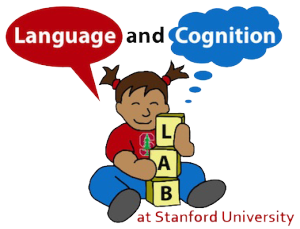
\includegraphics{figs/image-1} 

}

\caption[One column image]{One column image.}\label{fig:image}
\end{figure}
\end{CodeChunk}

\hypertarget{r-plots}{%
\subsection{R Plots}\label{r-plots}}

You can use R chunks directly to plot graphs. And you can use latex
floats in the fig.pos chunk option to have more control over the
location of your plot on the page. For more information on latex
placement specifiers see
\textbf{\href{https://en.wikibooks.org/wiki/LaTeX/Floats,_Figures_and_Captions}{here}}

\begin{CodeChunk}
\begin{figure}[H]

{\centering 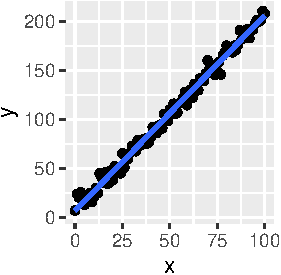
\includegraphics{figs/plot-1} 

}

\caption[R plot]{R plot}\label{fig:plot}
\end{figure}
\end{CodeChunk}

\hypertarget{tables}{%
\subsection{Tables}\label{tables}}

Number tables consecutively; place the table number and title (in 10
point) above the table with one line space above the caption and one
line space below it, as in Table 1. You may float tables to the top or
bottom of a column, set wide tables across both columns.

You can use the xtable function in the xtable package.

\begin{table}[H]
\centering
\begin{tabular}{rrrrr}
  \hline
 & Estimate & Std. Error & t value & Pr($>$$|$t$|$) \\ 
  \hline
(Intercept) & -0.08 & 0.11 & -0.7 & 0.47 \\ 
  x & 1.96 & 0.11 & 18.0 & 0.00 \\ 
   \hline
\end{tabular}
\caption{This table prints across one column.} 
\end{table}

\hypertarget{acknowledgements}{%
\section{Acknowledgements}\label{acknowledgements}}

Place acknowledgments (including funding information) in a section at
the end of the paper.

\hypertarget{references}{%
\section{References}\label{references}}

\setlength{\parindent}{-0.1in} 
\setlength{\leftskip}{0.125in}

\noindent

\hypertarget{refs}{}
\leavevmode\hypertarget{ref-ChalnickBillman1988a}{}%
Chalnick, A., \& Billman, D. (1988). Unsupervised learning of
correlational structure. In \emph{Proceedings of the tenth annual
conference of the cognitive science society} (pp. 510--516). Hillsdale,
NJ: Lawrence Erlbaum Associates.

\leavevmode\hypertarget{ref-NewellSimon1972a}{}%
Newell, A., \& Simon, H. A. (1972). \emph{Human problem solving}.
Englewood Cliffs, NJ: Prentice-Hall.

\bibliographystyle{apacite}


\end{document}
